\documentclass[11pt,a4paper]{article}
\usepackage[english]{babel}

\usepackage{verbatim}


\usepackage{amsmath,amsfonts, amssymb, amsthm}
\usepackage{amsbsy}
\usepackage[shortlabels]{enumitem}
\usepackage{makeidx}
\usepackage{graphicx}
\usepackage[dvipsnames]{xcolor}
\makeindex

\usepackage[top=2cm, bottom=2.5cm, inner=2cm, outer=2cm]{geometry}

\usepackage[colorlinks,linkcolor=red,citecolor=green,urlcolor=blue,hypertexnames=true]{hyperref}

\usepackage{tikz}

\newcommand{\lvec}{$v_1,\cdots, v_n$}

\usepackage{xcolor}
\newcommand{\pozor}[1]{\textcolor{red}{#1}}
\newcommand{\CR}{\textcolor{red}}

\newcommand{\R}{\mathbb R}
\newcommand{\N}{\mathbb N}
\newcommand{\Z}{\mathbb Z}
\newcommand{\C}{\mathbb C}
\newcommand{\Q}{\mathbb Q}

\newenvironment{primer}[1][]{\begin{primer*}[#1]\renewcommand*{\qedsymbol}{$\diamondsuit$}\pushQED{\qed}}{\popQED\end{primer*}}


\theoremstyle{plain}
\newtheorem{theorem}{Theorem}[section]
\newtheorem{proposition}[theorem]{Proposition}
\newtheorem{lemma}[theorem]{Lemma}

\theoremstyle{definition}
\newtheorem{definition}[theorem]{Definition}

\theoremstyle{plain}
\newtheorem{izrek}{Izrek}[section]
\newtheorem{trditev}[izrek]{Trditev}
\newtheorem{lema}[izrek]{Lema}

\theoremstyle{definition}
\newtheorem{definicija}[izrek]{Definicija}

\title{Osnove programa \LaTeX}
\author{Tea Strekelj \and ?? \and ??}
\date{\today}

\begin{document}

\maketitle
\thispagestyle{empty}
\newpage

\begin{abstract}
	Kratek povzetek vsebine.
\end{abstract}

\newpage
	
	\section{Beginning}\label{sec:beg}

	Moja\ \  datoteka   
	
	``datoteka".
	
	\$
	
	\%
	
	%moj komentar
	
	\begin{comment}
		fhjkbfjklagjsegneksio
	\end{comment}
	
	\begin{verbatim}
		Pisalni stroj    $
	\end{verbatim}
	
	
	\begin{definicija}
		Prva definicija.
	\end{definicija}
	
	\begin{izrek}\label{izr:pitagora}
		Velja $a^2+b^2=c^2.$
	\end{izrek}
	\index{izrek}
	
	\begin{proof}
		Dokaz zgornjega izreka. 
	\end{proof}
	
	Glej izrek \ref{izr:pitagora}.
	
	\begin{proof}
		Dokaz zgornjega izreka. Upoštevaj
			\begin{equation*}
			x^2+y^3+4 = 5z.\qedhere
			\end{equation*}
	\end{proof}
	
	
	
	\begin{tikzpicture}
		\draw (1,2) -- (3,5) -- (0,5) -- cycle;
		\draw[->] (1,2) -- (4,2);
	\end{tikzpicture}
	
	\begin{tikzpicture}
		\draw[->] (0,0) .. controls (1,1) and (3,1) .. (4,0);
	\end{tikzpicture}
	
	$\N, \R, \C, \Q,\Z$
	
	
	Moja enačba $x=2.$ Lahko tudi v display style:
	$$
	x^2+y^3+4 = 5z.
	$$
	Glej razdelek \ref{sec:beg}.
	\index{dollars}
	Na ta način je okoli enačbe več prostora. Običajen x,y,z. 
	
	Tudi x izven displaya pišemo kot $x.$
	
	\begin{trditev}
			Okolje equation za oštevilčevanje enačb:
		\begin{equation}\label{eq:pitagora}
			a^2+b^2=c^2.
		\end{equation}
	\end{trditev}
	

	
Glej enačbo \eqref{eq:pitagora}. Obstaja tudi \ref{eq:pitagora}, ki pa ga ne uporabljamo za enačbe, temveč za izreke, trditve, itd.

\section{Enačbe}
\index{enačbe}

\begin{izrek}
\begin{equation} \tag{Einstein}
	E =mc^2
\end{equation}
\end{izrek}



\begin{equation*}
	s = vt
\end{equation*}
\index{equation!no-number}
deluje isto kot 2x2 dolarja.	

$$
Moja \  enacba \text{ Pokončen $a$ text}
$$


\begin{align*}
	x^w+z=y \\
	c^6+7u=a\\
	f+g=h
\end{align*}
\index{align}
	
	
	$\lambda, \alpha, \beta, \gamma, \Gamma, \Lambda, \pi, \phi, \varphi$
	
	
	$$
	a^4, a^{b^5}, a^45, a^{45}
	$$
	
	$$
	a_n, a_34, a_{34}, a_{n_k}
	$$
	
%$$
%a > b, 3 \geq 3, 3 \neq 4,3 \not = 4, M \subseteq N, M \not \subset N, G \approx H, G \cong H, \pi \approx 3, N \supseteq M
%$$
%
%$$
%a \in A, a \not \in A, a \notin A
%$$
%
%$$
%A = \{ x \mid x \geq 0\} = \{a \ | \ a \geq 0\}
%$$
%
%$$
%\sqrt{2x^2 + y^2-1}, \sqrt{\frac23}, \sqrt[3]{45}, \sqrt[n]{x^n}, \surd{456}
%$$
%
%$$
%f: A \to B, \quad f:A \rightarrow B,\quad f: a \mapsto f(a), f\colon A \to B
%$$
%
%$$
%A \implies B, \quad  A \Longrightarrow B, \quad A \Leftrightarrow B, A \Longleftrightarrow B, A \iff B
%$$
%
%$$
%\lim_{x \searrow 0} \sqrt{x}, \quad \lim_{y \nearrow 5} (y^5-4y+7)
%$$
%
%$$
%... \quad \text{ or } \quad \ldots
%$$
%
%$$
%n! = 1 \cdot 2 \cdots  n,\quad  1 + \cdots +n, \quad k = 1,\ldots, n
%$$
%$$
%\vdots \quad \ddots
%$$
%
%$$
%n = \underbrace{1 + \cdots + 1}_{n \text{ times}} = \overbrace{1 + \cdots + 1}^{n \text{ times}}
%$$
%
%$$
%f'(x), f^\prime(x), f''(x), f^{\prime \prime}(x)
%$$
%
%
%$$
%lim_{x\to 4} x^6, \quad \lim_{x\to 6} f(x) \quad \text{lim}_{x\to 7} f(x)
%$$
%
%$$
%\frac12, \frac{23}{45}, \frac{\text{up}}{\text{down}}
%$$
%
%$$
%x^2 \stackrel{(*)}{=} y^2+z^2
%$$
%
%$$
%\int_{-\frac{\pi}{2}}^{\frac{\pi}{2}} f(x)\, dx
%$$
%
%$$
%\sum_{n=1}^\infty \frac{1}{n} = \infty
%$$
%
%$$
%\sum_{\substack{n=0,\\ n \text{ not divisible by } 2}}^{25} n^2+3
%$$
%
%$$
%\left|\left[\left\{\left( \sum_{\substack{1 \leq i,j \leq n,\\ i \neq j}} i-j \right)\right\}\right]\right|
%$$
%
%$$
%\Bigg(\bigg(\Big(\big(\left(\int_0^2 x^2\, dx \right)\big)\Big)\bigg)\Bigg)
%$$
%
%
%$$
%|| z|| \neq \|z\|
%$$
%
%$$\big\langle x, y \big\rangle = x_1y_1 + \cdots x_ny_n$$
%
%\begin{align*}
%	x &= 2y + 6z \\
%	5y &= 6z + 7t + b\\
%	4z + 3 y &= 3t + 9k
%\end{align*}
%
%\begin{align*}
%	&x = 2y + 6z \\
%	&5y = 6z + 7t + b\\
%	&4z + 3 y = 3t + 9k
%\end{align*}
%
%
%\begin{align}
%	&x = 2y + 6z \nonumber \\
%	&5y = 6z + 7t + b\\
%	&4z + 3 y = 3t + 9k \nonumber
%\end{align}
%
%
%
%$$
%\begin{matrix}
%	1& 2 \\
%	3 & 4
%\end{matrix} \quad
%\begin{pmatrix}
%	1& 2 \\
%	3 & 4
%\end{pmatrix}\quad
%\begin{bmatrix}
%	1& 2 \\
%	3 & 4
%\end{bmatrix} \quad
%\begin{vmatrix}
%	1& 2 \\
%	3 & 4
%\end{vmatrix}
%$$
%
%
%$$
%\begin{pmatrix}
%	a_{11} & \cdots & a_{1n}\\
%	\vdots & \ddots & \vdots\\
%	a_{n1} & \cdots & a_{nn}
%\end{pmatrix}
%$$
%
%$$
%f(x) =
%\begin{cases}
%	2x; & \text{ if } x \geq 0\\
%	3x; & \text{ if } x < 0 
%\end{cases}
%$$
%
%\begin{align}
%f(x) =
%\begin{cases}
%	2x\ \mid & x \geq 0\\
%	3x\ \mid & x < 0 
%\end{cases}
%\end{align}
%
%Let $\mathcal{A}$ be an algebra. Let $\mathbb{N}$ denote the set of positive integers. Let $\mathbb{R}$ be the real numbers. We also have $\mathbb{C,Q}.$ The mathfrak font is sometimes used to denote the imaginary unit: $z = x + \mathfrak{i}y.$
%Let $\boldsymbol{\lambda}$ be a partition. 

\section{Simboli}
$$
a > b, a \geq b, a \leq b, A \subset B, A \not \subset B, A \subseteq B, A \supset B
$$

$$
a \in A, a \not \in A, a \notin A, A \preceq B, A \succeq B, a = b, a \neq b, a \approx , G \cong H
$$


$$
A = \{ x \mid x \geq 0 \} = \{ x \ | \ x \geq 0  \}
$$

$$
\sqrt{x^2+3y+z^{2^n}}, \quad \sqrt{x+2} \quad \sqrt{\frac23}, \quad \sqrt[n]{a^2+b^2}, \quad \sqrt[3]{45}
$$

$$
f: X \to Y,\quad f \colon X \to Y, \quad f\colon x \mapsto x^2
$$
\subsection{Logični simboli}\label{subsec:log}
$$
A \implies B, \quad A \Longrightarrow B,\quad A \iff B,\quad A \Longleftrightarrow B
$$

\begin{figure}
\begin{center}
\setlength \fboxsep{0pt}
\setlength \fboxrule{2pt}
\fbox{\includegraphics[scale=0.6]{cvx}}
\end{center}
\caption{Konveksnost}
\label{fig:cvx}
\end{figure}

Glej sliko \ref{fig:cvx}.

\index{logični simboli}

$$
\lim_{x \nearrow 0} f(x) \quad \lim_{x \searrow 4} g(x)
$$

$$
k=1,\ldots,n \quad n! = 1\cdot 2 \cdots n \quad k =1,...,n
$$


$$
n = \underbrace{1 + \cdots + 1}_{n \text{-krat}} = \overbrace{1 + \cdots + 1}^{n \text{-krat}}
$$

$$
lim_{x \to 1} f(x) \quad \lim_{x \to 1} f(x) \quad \sin(\pi) \quad \cos(2\pi)
$$

$$
\min_{x \geq 0} x^2  \quad \sup_{1 \leq x \leq 2} g(x) \quad \det(\lambda I)
$$

$$
\frac12, \frac{x^2+3y +7z}{y^2-5z+3x}, \sqrt{\frac{y^{15}-3}{2x}}
$$

$$
c^2 \stackrel{(1)}{=} a^2+b^2
$$
\subsection{Analiza}
$$
\int_0^1 \sin(\pi x)dx = \int_0^1 \sin(\pi x)\,dx
$$
\subsubsection{Vsote}

$$
\sum_{n=1}^\infty \frac{1}{n} \quad \sum_{k=1}^n k^2
$$


$$
\sum_{\substack{1 \leq i,j \leq n \\ i \neq j}} i-j
$$

$$
\Bigg( \bigg( \Big( \big( ( \left(\sum_{n=1}^\infty \frac{1}{n}\right) ) \big) \Big) \bigg) \Bigg)
$$

$$
\langle x,y \rangle = x_1y_1+\cdots x_ny_n
$$

\begin{align}
	x &= 3y+5z \\
	4x + 3y &= 6z+8w\\
	6y+5x &= 2w + 19 + 15z
\end{align}

\begin{align}
	&x = 3y+5z \nonumber\\
	&4x + 3y = 6z+8w\\
	&6y+5x = 2w + 19 + 15z \nonumber
\end{align}


$$
\begin{pmatrix}
	1 & 2 & 3 \\
	4 & 5 & 6 \\
	7 & 8 & 9
\end{pmatrix}
$$
\index{matrix}

\begin{equation}
	\begin{bmatrix}
		a & b \\
		c & d
	\end{bmatrix}
\end{equation}

\begin{align*}
	\begin{vmatrix}
		a_{11} & \cdots & a_{1n}\\
		\vdots & \ddots & \vdots \\
		a_{n1} & \cdots & a_{nn}
	\end{vmatrix}
\end{align*}

$$
f(x) = 
\begin{cases}
	x^2 & \text{ if } x < -1\\
	2x+3 & \text{ if }  -1 \leq x \leq 4\\
	5x & \text{ if } x > 4
\end{cases}
$$
\index{cases}
$$
f(x) = 
\begin{cases}
	x^2 &\mid  x < -1\\
	2x+3  &\mid -1 \leq x \leq 4\\
	5x &\mid  x > 4
\end{cases}
$$


Naj $\mathbb{N}$ označuje naravna števila, $\mathbb{R}$ realna, $\mathbb{C}$ kompleksna in $\mathbb{Q}$ racionalna števila.

Naj bo $\mathcal{A}$ algebra\footnote{Torej vektorski prostor z množenjem.}. Naj bo $\mathfrak{A}$ algebra.
Označimo $z = x + \mathfrak{i} y.$ Glej tudi podrazdelek \ref{subsec:log}.

$$
\mathbf{\lambda}, \boldsymbol{\lambda}
$$

\section{Mathematical exercises}

Continuing from Section. See page \pageref{sec:beg}.

\begin{enumerate}
	\item First
	\item second
\end{enumerate}

\begin{itemize}
	\item first
	\item second
\end{itemize}

\begin{enumerate}[(a)]
	\item 
	\item 
	\item
\end{enumerate}

\begin{enumerate}[(i)]
	\item 
	\item 
	\item
	\item
\end{enumerate}

\begin{definition}
	The style of definitions is different.
\end{definition}

\begin{theorem}\label{thm:first}
	state your theorem here.
\end{theorem}
\index{theorem}

\begin{proof}
	Proof of above theorem here.
	\begin{equation*}
		a^2+b^2=c^2       \qedhere
	\end{equation*}
\end{proof}

\begin{table}
\begin{center}
\begin{tabular}{|c|r|l|}
	\hline
	1 & 2 & 3 \\
	\cline{2-3}
	4 & 5 & 6\\
	\hline \hline
	\multicolumn{2}{|c|}{78} & 9\\
	\hline
\end{tabular}	
\end{center}
\caption{Tabela števil}
\label{tab:st}
\end{table}

\begin{figure}[h]
	\centering
	% Left Side Minipage
	\begin{minipage}{0.45\textwidth}
		\centering
		%			\includegraphics[width=\linewidth]{image1.jpg}
		\caption{Caption for Image 1}
	\end{minipage}
	\hfill % Adds horizontal space between the two minipages
	% Right Side Minipage
	\begin{minipage}{0.45\textwidth}
		\centering
		%			\includegraphics[width=\linewidth]{image2.jpg}
		\caption{Caption for Image 2}
	\end{minipage}
\end{figure}

\noindent
\begin{minipage}[c]{0.5\textwidth}
	\section*{Description}
	This text is contained within a minipage that takes up exactly 
	half of the page width. Because the alignment is set to [c], 
	it will stay centered relative to the image on the right.
\end{minipage}
\hfill
\begin{minipage}[c]{0.4\textwidth}
	\centering
	%	\includegraphics[width=\linewidth]{diagram.png}
\end{minipage}

\CR{Here is my note.}

\textcolor{blue!80}{EXAMPLE}
\textcolor{blue!80!black}{EXAMPLE}
\textcolor{blue!20!black!30!green}{EXAMPLE}
\textcolor{green}{EXAMPLE}
\textcolor{orange}{EXAMPLE}
\textcolor{yellow!50!}{EXAMPLE}


Glej tabelo \ref{tab:st}

\url{https://e.famnit.upr.si/course/view.php?id=7087}\\
\href{https://e.famnit.upr.si/course/view.php?id=7087}{For moodle click here}

\vspace{2cm}

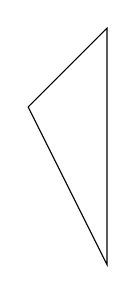
\begin{tikzpicture}
	\draw (1,1)--(2,2)--(2,-1)--cycle;
\end{tikzpicture}


\begin{tikzpicture}
	\draw (0,0) .. controls (1,1) and (3,1).. (4,0);
\end{tikzpicture}

\vspace{3cm}

The following follows from Theorem \ref{thm:first}. The proof can be found in \cite{rudin} or \cite{rudin2}. See also \cite[Section 3]{rudin} or \cite[Theorem 2.6]{rudin2}. 

\begin{proposition}
	first proposition
\end{proposition}

\tableofcontents

\printindex


\begin{thebibliography}{99}
	\bibitem{rudin} Rudin,  Analysis 1, 1990.
	\bibitem[Rud92]{rudin2} Rudin, Functional Analysis, 1992.
\end{thebibliography}











	
\end{document}